\documentclass[a3]{swfuexam}

\swfusetup{%
  Yfrom=1237,%
  Yto=1238,%
  Term=1,%
  Course={打狗棒法},%
  AB=A,%
  Group={丐帮1236级乙班},%
  EXtype={闭卷},%
  EXtime={120},%
  Lecturer={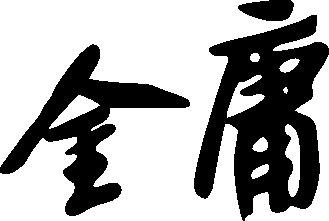
\includegraphics[height=1cm]{jinyong}},%
}

\begin{document}
\SWFCbinding
\SWFCheader

\section{填空题 ( $3\times2=6$分 )}

\begin{enumerate}
\item 三十六路打狗棒法是\blank{6em}所创,历来是前任帮主传后任帮主,决不传给第二个人,丐帮
  第\blank{6em}任帮主的武功尤胜开帮祖师,他在这路棒法中更加入无数奥妙变化,数百年来,丐帮逢到危难关头,
  帮主亲自出马,往往便仗这打狗棒法除奸杀敌,震慑群邪。
\item 《打狗棒法》一书的作者是\blank{6em}。
\end{enumerate}
% \Clearpage
\vfill
\section{单项选择题 ($1\times5=5$分)}
\begin{enumerate}
\item 打狗棒是一根通體碧綠,精光溜滑的\blank{2em}棒。
  \begin{tasks}(4)
    \task 玉
    \task 铁
    \task 铜
    \task 竹
  \end{tasks}
\end{enumerate}
% \Clearpage
\vfill
\section{判断题 ( $4\times2=8$分 )}
\textbf{请在(\blank{1em})內标记(\underline{$\checkmark$})或者(\underline{$\times$}).}
\begin{enumerate}
\item (\blank{1em}) 杨过会使打狗棒法。
\item (\blank{1em}) 周伯通会使打狗棒法。
\item (\blank{1em}) 打狗棒法属于内家功夫。
\item (\blank{1em}) 西毒欧阳锋死于北丐洪七公棒下。
\end{enumerate}
\vfill
%\Clearpage
\section{名词解释 ($2\times5=10$分)}
\subsection*{惡狗攔路}
\begin{itemize}
\item[答:] 
\end{itemize}
\vspace{20em}

%\vfill
\subsection*{棒打雙犬}
\begin{itemize}
\item[答:] 
\end{itemize}

\vspace{20em}

\vfill%\Clearpage
\section{简答题 ( $2\times 5=10$分 )}

\subsection{如遇敌人执刀正面劈来,当用棒法中的哪一招应对?为什么?}
\begin{itemize}
\item[答:] 
\end{itemize}

\vspace{20em}
\vfill%\Clearpage
\subsection{打狗棒丢失当如何办?}
\begin{itemize}
\item[答:] 
\end{itemize}

\vspace{20em}
\vfill%\Clearpage
\section{问答题 ($1\times{}20=20$分)}
\subsection{请详细阐述打狗棒法厉害还是降龙十八掌厉害?}
\begin{itemize}
\item[答:] 
\end{itemize}

\vspace{20em}

\end{document}

%%% Local Variables: 
%%% mode: latex
%%% TeX-master: t
%%% End: 
